% Pulse-Echo Azimuthal Simulation: the simulation manual.
%
% Build with build.ps1 (XeLaTeX, two passes), or:
%   xelatex simulation-manual.tex && xelatex simulation-manual.tex
%
% Each chapter lives in its own numbered folder; each section is a
% separate .tex file, \input from the chapter list below, so individual
% sections can be updated without touching the rest of the document.

\documentclass[11pt,a4paper]{report}

\usepackage{geometry}
\geometry{margin=2.5cm}
\usepackage{graphicx}
\usepackage{booktabs}
\usepackage{tabularx}
\usepackage{amsmath}
\usepackage{siunitx}
\usepackage[hidelinks,
  pdftitle={Pulse-Echo Azimuthal Simulation: Manual},
  pdfauthor={Jerome Graves},
  pdfsubject={Simulation and inversion of rotational pulse-echo ultrasound on polycrystalline ice}]{hyperref}
\usepackage{xcolor}
\usepackage{listings}

\lstset{basicstyle=\ttfamily\small, frame=single, framerule=0.3pt,
        columns=fullflexible, keepspaces=true, breaklines=true,
        xleftmargin=0.5em, aboveskip=0.8em, belowskip=0.8em}

\newcommand{\cmd}[1]{\texttt{#1}}

\begin{document}

\begin{titlepage}
  \centering
  \vspace*{1cm}
  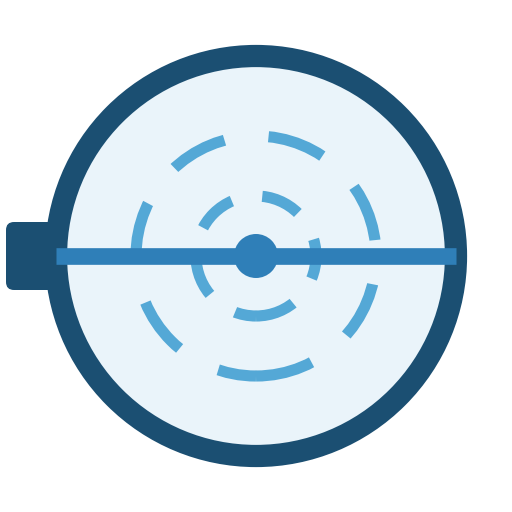
\includegraphics[width=2.2cm]{figures/logo.png}\\[1.2em]
  {\Huge Pulse-Echo Azimuthal Simulation}\\[0.6em]
  {\Large Simulation Manual}\\[2em]
  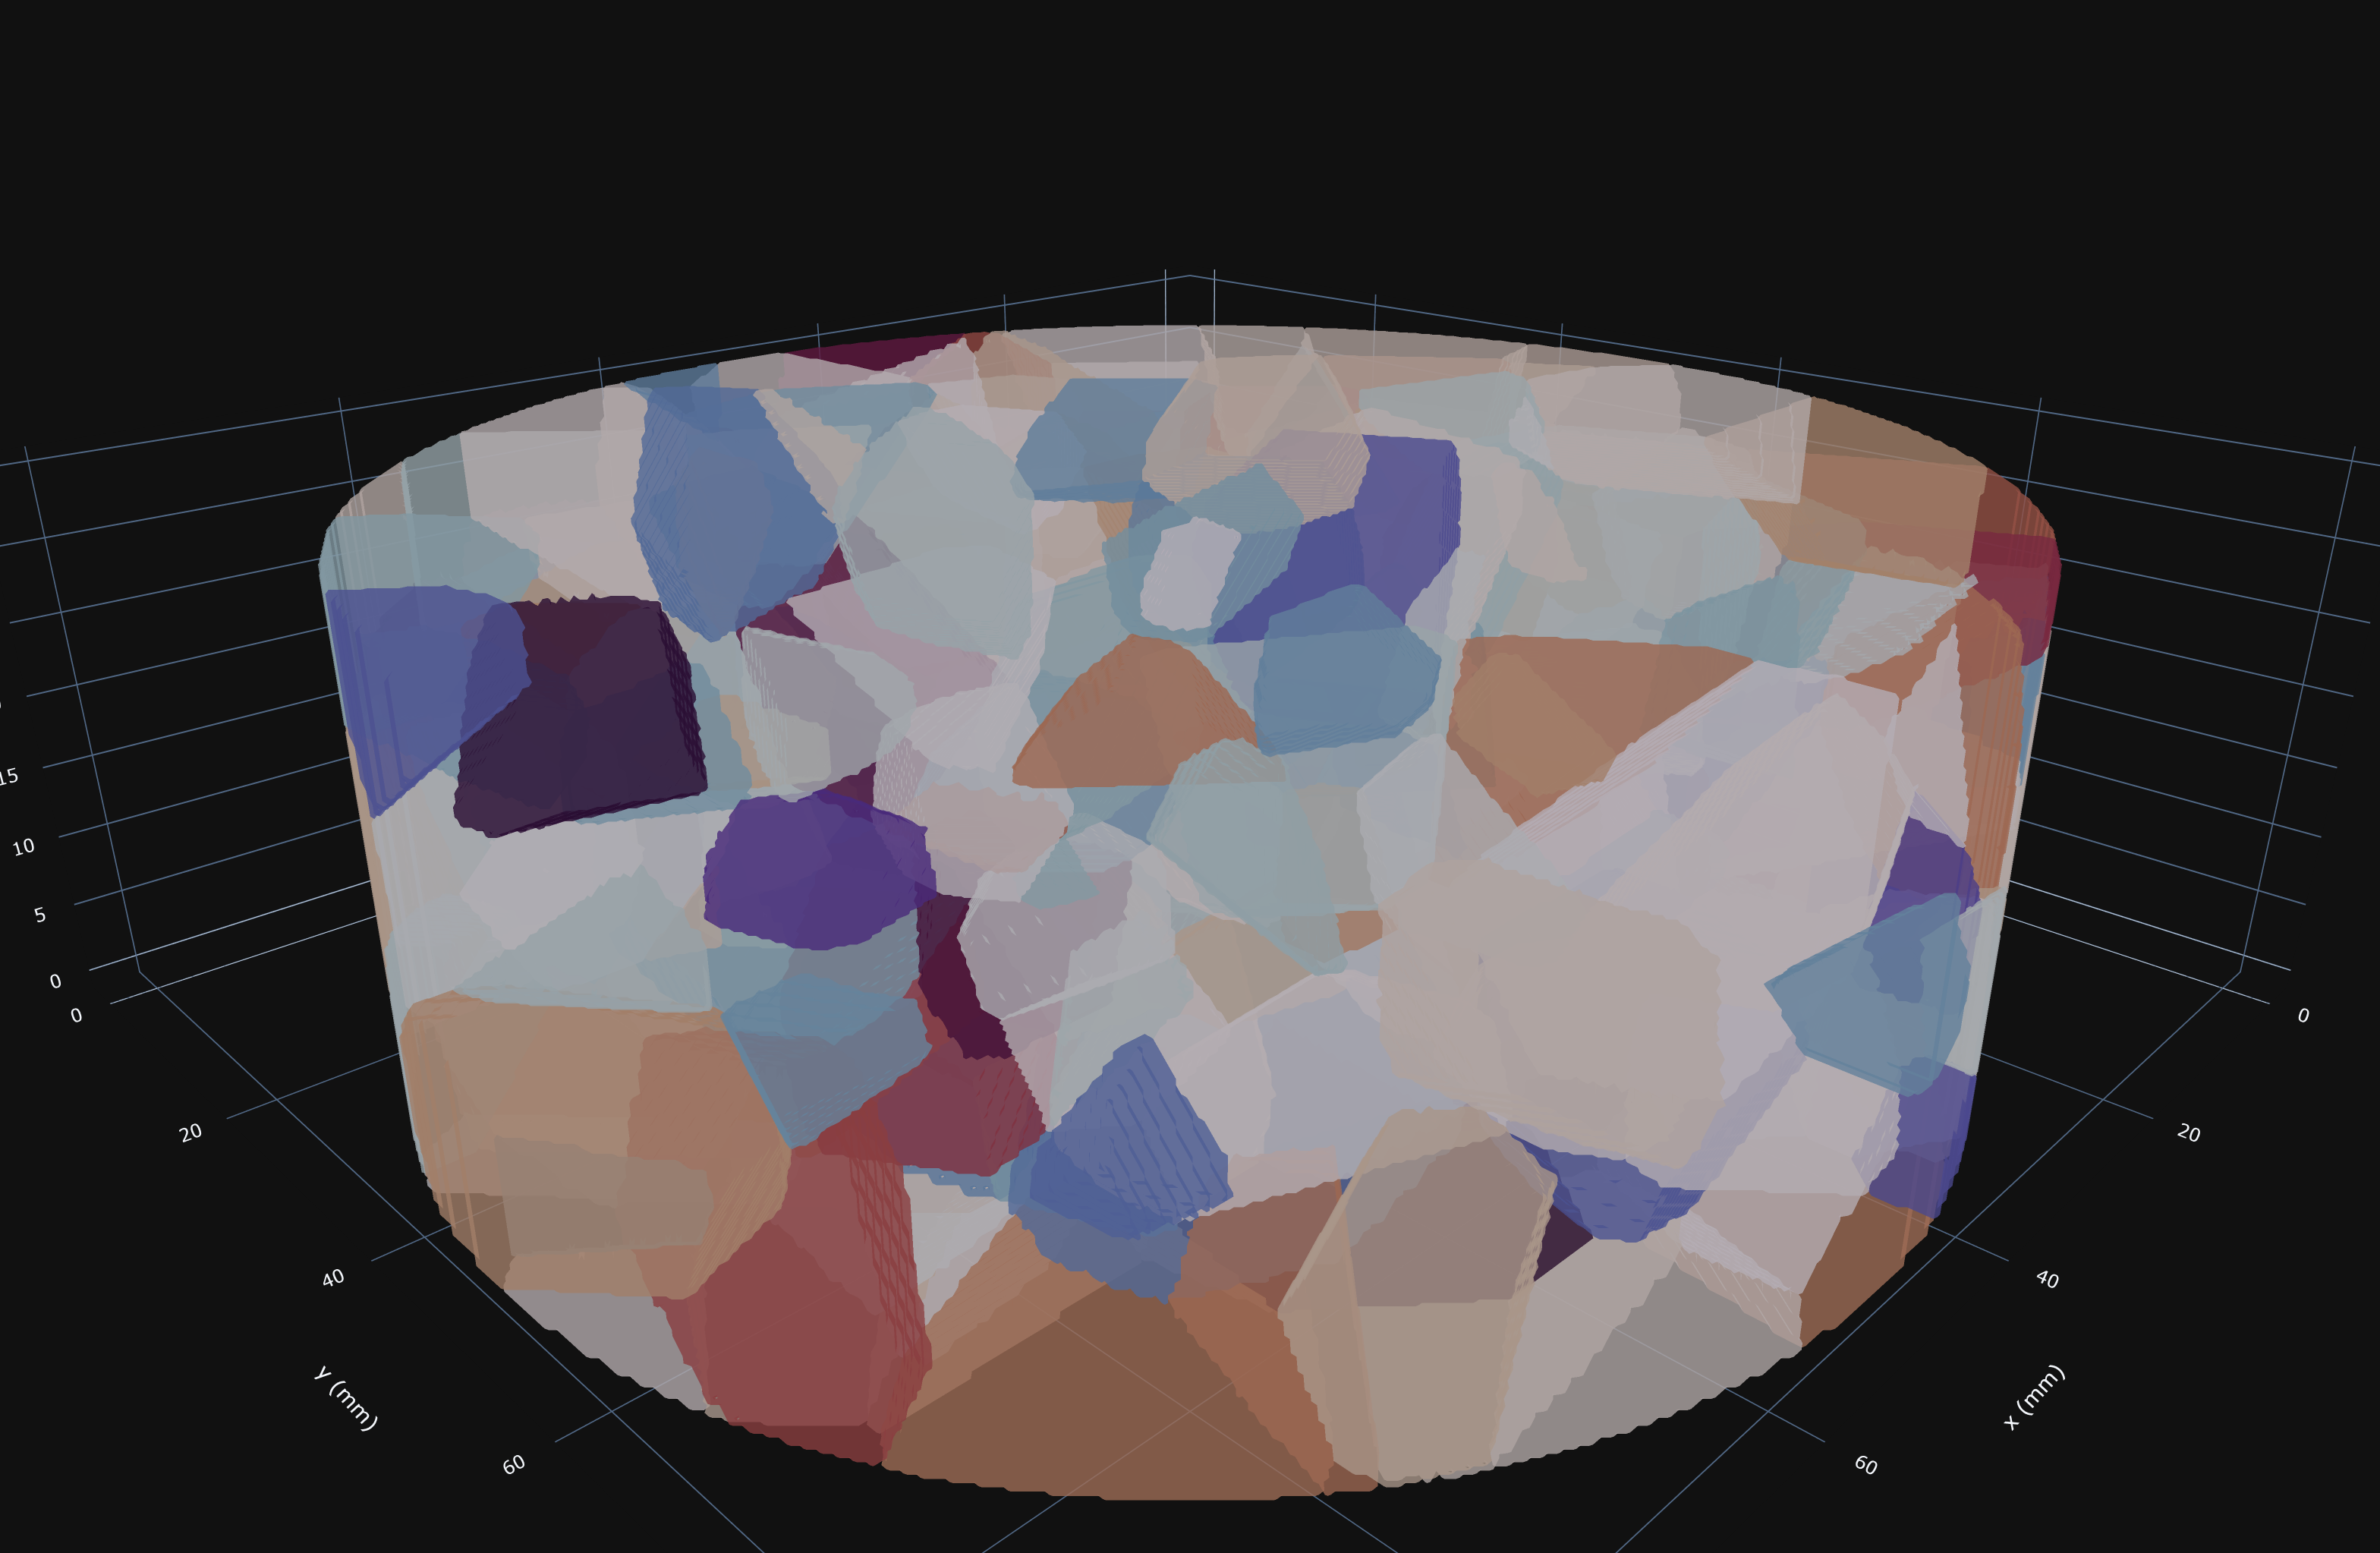
\includegraphics[width=0.95\textwidth]{figures/specimen-3d.png}\\
  \vfill
  {\large Jerome Graves}\\[0.3em]
  \href{https://jeromegraves.com}{jeromegraves.com}\\[0.4em]
  \today
\end{titlepage}

\tableofcontents

\chapter{Overview}\label{ch:overview}
\section{What this software is}

This repository is the digital twin of the pulse-echo azimuthal
measurement: a rotational single-transducer ultrasound method that
recovers the crystal orientation fabric (COF) of a polycrystalline ice
disk from the azimuthal variation of diametral sound velocity. The
physical instrument is documented in its own repository and manual;
this codebase answers the questions an instrument cannot: what should
the measurement see for a known fabric, which parts of the received
signal carry fabric information, how do acquisition errors corrupt it,
and how well can the fabric be recovered.

The pipeline has four stages, mirrored by the GUI tabs:

\begin{enumerate}
  \item \textbf{Specimen.} Build a synthetic disk: Voronoi grain
    structure with controlled size distribution, and a Watson
    orientation distribution with controlled strength and mean
    direction (Chapter~\ref{ch:specimen}).
  \item \textbf{Forward model.} Propagate pulses through the disk,
    either with the fast ray model (interactive) or the label-indexed
    anisotropic FDTD solver (full-wave, GPU), which is itself
    validated against an independent finite-element solver
    (Chapter~\ref{ch:forward}).
  \item \textbf{Acquisition and errors.} Simulate the rotational
    acquisition of the physical machine, with its error model
    (Chapter~\ref{ch:acquisition}).
  \item \textbf{Analysis and inversion.} Recover the fabric from the
    simulated traces and quantify what is and is not recoverable
    (Chapter~\ref{ch:analysis}).
\end{enumerate}

The repository doubles as the evidence base for the journal
manuscript on the method. The working convention throughout: every
number quoted in the paper traces to a module here, and the expected
output is recorded in that module's docstring. Negative results are
kept deliberately, because ruling a signal path out is as much a part
of the argument as ruling one in.

\section{Quick start}

\subsection{The GUI}

Double-click \cmd{Run Simulation GUI.bat} in the repository root. The
first launch installs a private Python runtime into \cmd{gui/runtime/}
(internet required, a few minutes) with the repository's pinned
package versions plus the GUI extras; afterwards it starts offline,
creates an icon-bearing shortcut, and opens at
\cmd{http://localhost:8552}.

The studio walks the pipeline as a gated workflow: Specimen \&
Fabric, Probe \& Excitation, Error model, then Acquisition; the
Backscatter and COF reconstruction tabs unlock once acquired data
exists. The FW sweep tab drives the resumable full-wave azimuth sweep
engine.

Everything interactive (specimen builder, ray forward model, error
model, reconstruction views) runs on CPU. New full-wave runs need
CUDA and cupy in the running Python environment; the GUI detects the
backend by inspection and reports it under the title.

\subsection{Reproducing a stored result}

No GPU is needed to reproduce any analysis in the paper. For example,
the finite-element cross-check of direct-arrival attenuation:

\begin{lstlisting}
cd sim/analysis
python fe_direct_attenuation.py
\end{lstlisting}

prints a table of the five cross-check rounds; the expected values,
including the 0.027 dB solver agreement for the 6 to 15 mm placement,
are recorded in the module docstring. Every cited module follows the
same pattern: run it from its own directory, compare the printed
numbers with the docstring.

\section{The reproduction contract}

The version pins in \cmd{requirements.txt} are deliberate and strict:
numpy and scipy are pinned to the exact versions under which the
stored results were produced. The analysis layer contains
bit-exactness gates that compare recomputed arrays against archived
ones at zero tolerance. Other library versions move floating point at
the $10^{-13}$ level, which is physically meaningless but trips those
gates by design; the gates exist precisely to detect that anything at
all has changed. With the pinned versions every gate returns zero;
with other versions, expect agreement at the $10^{-12}$ level and two
modules stopping at their gate on purpose.

Large artefacts follow a strict rule: no bulky binary ever enters git
history. Solver meshes and sweep outputs are regenerable and live
outside version control; the tracked exceptions are a handful of
kilobyte-scale trace archives that are the only raw evidence behind
specific paper claims, kept so those claims can be checked without
rebuilding a multi-hundred-megabyte mesh. \cmd{DATA\_MANIFEST.md} records what
data lives where.


\chapter{Specimen and fabric model}\label{ch:specimen}
\section{Grain structure}

A specimen is a disk (default \SI{100}{mm} diameter, \SI{35}{mm}
thick) filled with a Voronoi tessellation of grains. The builder
(\cmd{sim/core/specimen.py}, \cmd{DiskSpecimen}) controls grain count,
the spread of grain sizes about the mean (a coefficient of variation
on the seed weighting), and the random seed, so specimens are exactly
repeatable. The tessellation is rasterised onto the solver grid as a
label field: every cell carries the integer index of its grain, and
all per-grain properties (orientation, stiffness) are looked up
through that label. This label-indexed representation is what makes
the anisotropic solver practical: the stiffness tensor field never
exists in memory, only labels and a per-grain property table.

The builder also reports the diagnostics that matter physically:
achieved grain count and mean equivalent diameter, the orientation
tensor eigenvalues of the realised fabric, and the mean disorientation
across grain boundaries, which is the quantity that drives scattering
strength. The title page shows a 3D rendering of a 300-grain specimen
with each grain coloured by its in-plane c-axis azimuth;
Figure~\ref{fig:specimen-slice} shows the same specimen's mid-plane
slice.

\begin{figure}[htb]
  \centering
  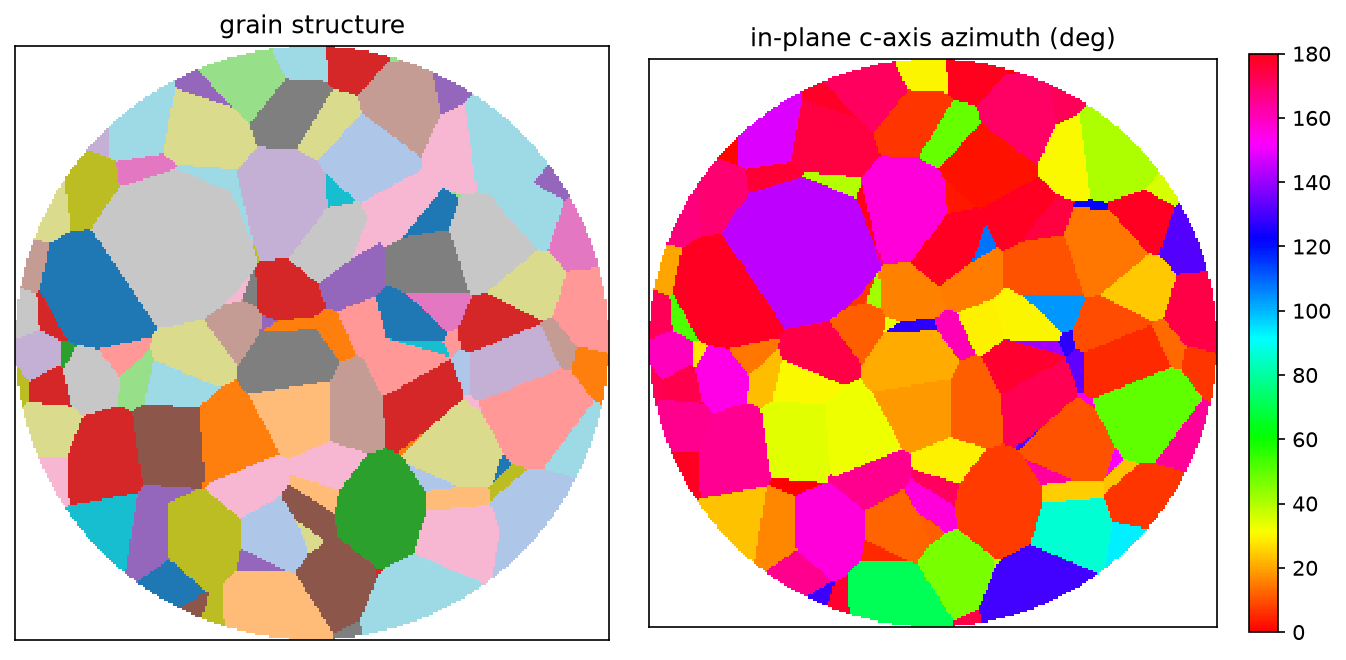
\includegraphics[width=0.95\textwidth]{figures/specimen-fabric.png}
  \caption{Mid-plane slice of a 300-grain specimen: grain structure
    (left) and the in-plane c-axis azimuth field (right).}
  \label{fig:specimen-slice}
\end{figure}

\section{Crystal orientation fabric}

Each grain's c-axis is drawn from a Watson distribution about a
chosen mean direction. The user-facing strength parameter is the
leading orientation-tensor eigenvalue $a_1$, the number ice thin
sections actually report: $a_1 = 1/3$ is random, $a_1 = 1$ a perfect
single maximum. The builder converts $a_1$ to the
Watson concentration $\kappa$ internally
(\cmd{kappa\_for\_eigenvalue}), so simulated fabrics are specified in
the same units as the field data they are compared against.

The mean direction is selectable. The default is in-plane, because
the azimuthal method reads the c-axis through second-harmonic
velocity patterns that an in-plane fabric produces directly; a
vertical (disk-normal) fabric is the method's null case and is
available precisely to demonstrate that. A spatial-correlation
control makes neighbouring grains more alike, which lowers boundary
disorientation and therefore scattering, independent of the bulk
fabric strength: bulk anisotropy and local disorder are deliberately
separate knobs, because the first drives the coherent $2\varphi$
velocity signal while the second drives the incoherent scattered
field.

Grain orientations, like the tessellation, are seed-repeatable, and
the realised (not target) orientation tensor is always reported,
since a 100-grain specimen realises the target distribution only
approximately. Figure~\ref{fig:pole} shows the realised fabric of the
title-page specimen on an equal-area pole figure.

\begin{figure}[htb]
  \centering
  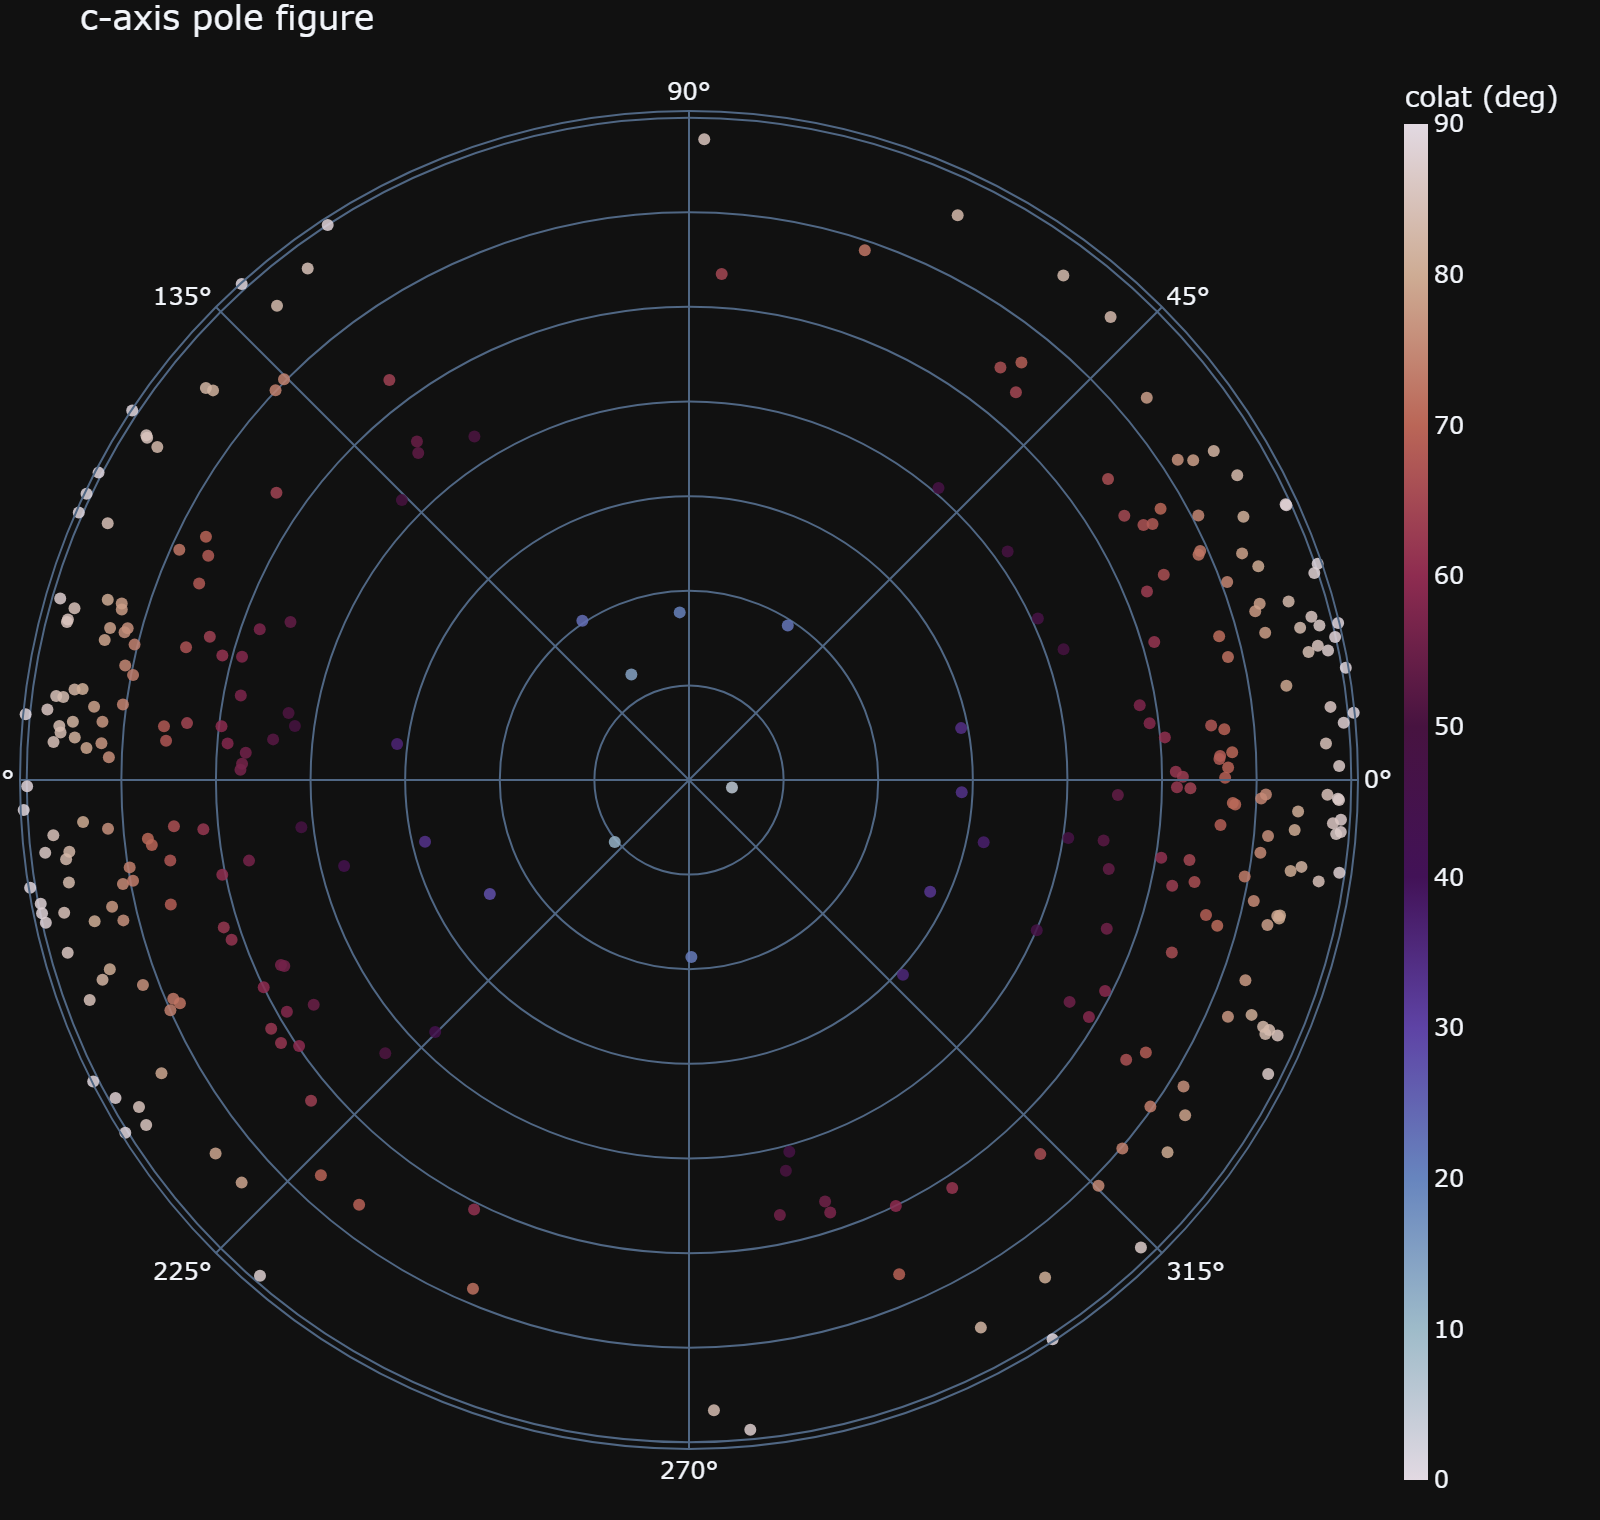
\includegraphics[width=0.55\textwidth]{figures/pole-figure.png}
  \caption{Equal-area (Schmidt) lower-hemisphere pole figure of the
    300-grain specimen at $a_1 = 0.70$ with an in-plane mean c-axis:
    a moderate single-maximum fabric.}
  \label{fig:pole}
\end{figure}


\chapter{Forward model and validation}\label{ch:forward}
\section{Solvers}

Three forward models coexist, used at different costs for different
questions:

\begin{description}
  \item[Ray model] (\cmd{sim/model/}, used by the studio). Pure
    numpy, interactive speed. Propagates diametral transits through
    the per-grain slowness field to predict travel times and the
    azimuthal velocity pattern. This is the model the inversion
    inverts, and the GUI's default backend.
  \item[Anisotropic FDTD] (\cmd{sim/core/fdtd.py}). The full-wave
    workhorse: a label-indexed elastic finite-difference solver in
    which every cell's stiffness comes from its grain's orientation.
    Runs on GPU through cupy; produces the synthetic pulse-echo
    traces the analysis layer consumes. A pseudospectral solver
    provides an independent numerical scheme for validation.
  \item[Finite-element arbiter] (\cmd{sim/fe\_crosscheck/}). A
    completely independent solver stack (its own mesher, elements
    and probes) used to adjudicate the FDTD results. When two
    unrelated discretisations of the same physics agree, the result
    is a property of the physics rather than the scheme.
\end{description}

The rotation machinery rotates the specimen rather than the probe,
matching the physical machine, and the bit-equivalence gate
(\cmd{validate\_labels.py}) guarantees the rotated label field feeds
the solver exactly the specimen the builder produced.

\section{Discretisation rules}

The production discretisation was fixed by convergence study, not
convention, and the settled rules are enforced as defaults:

\begin{itemize}
  \item at least 6 grid cells per wavelength at the source centre
    frequency,
  \item eighth-order spatial finite differences,
  \item boundary damping factor 0.02 in the absorbing layers.
\end{itemize}

Runs below these settings show visible numerical dispersion in the
coda and are suitable only for previews (the GUI's specimen preview
deliberately rasterises coarser, and says so). One historical trap is
documented for future users: early reference traces generated before
the absorbing-boundary settings were finalised carried a boundary
artefact that contaminated apparent scattering floors; the clean
reference set in \cmd{sim/ref/} postdates that fix, and the analysis
modules that measured the difference are kept as evidence.

\section{The validation chain}

The solver's license to be believed is a chain of checks, each stored
with its expected numbers in the corresponding module docstring:

\begin{enumerate}
  \item \textbf{Analytic checks} (\cmd{sim/validation/}): rotated
    staggered-grid behaviour and exact isotropic reflection
    coefficients against closed-form results.
  \item \textbf{Internal cross-scheme checks} (\cmd{sim/fw\_checks/}):
    the FDTD solver against the pseudospectral solver on shared
    problems, oblique-incidence validation, anisotropy checks and
    convergence studies, plus the crop and corridor licenses that
    justify the production domain sizes.
  \item \textbf{The independent arbiter} (\cmd{sim/fe\_crosscheck/}):
    five rounds of cross-checks against the finite-element stack.
    The headline result, reproducible from the archived traces
    without a GPU, is direct-arrival attenuation agreement between
    the two solvers to within hundredths of a decibel (0.014 to
    0.068 dB across the valid rounds).
\end{enumerate}

The chain is ordered by independence: each later stage shares less
with the solver under test than the one before. Chapter~\ref{ch:analysis}
leans on this: statements about what the scattered field does and
does not contain are only as good as the solver producing it.
Figure~\ref{fig:arbiter} shows the final arbiter round: the
grain-scattered field isolated by the same-specimen difference in
each solver, tracking between two discretisations that share nothing
but the physics.

\begin{figure}[htb]
  \centering
  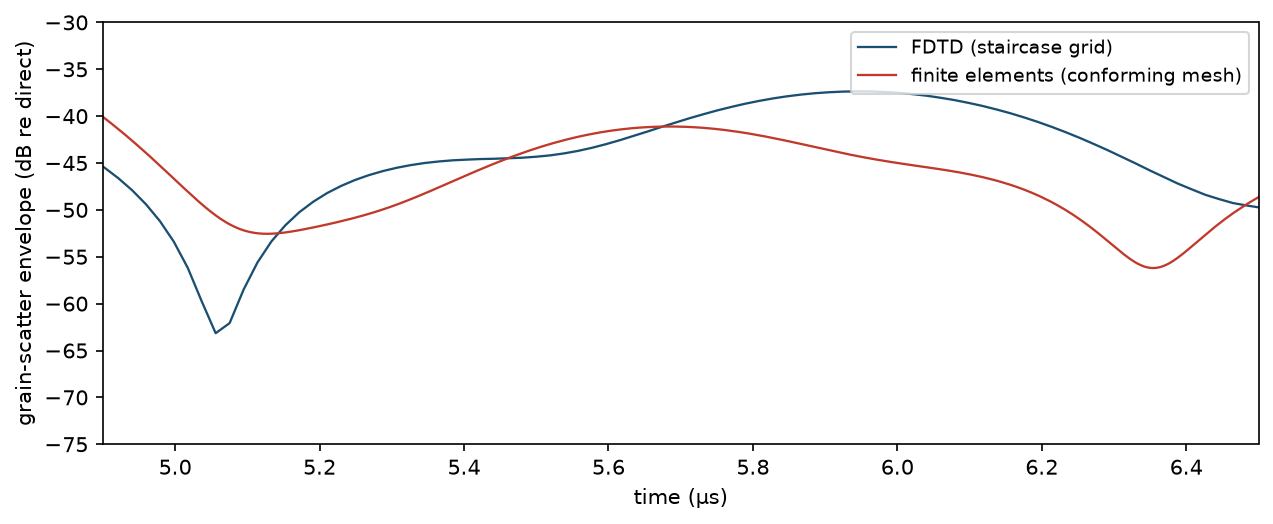
\includegraphics[width=0.95\textwidth]{figures/fe-arbiter.png}
  \caption{The passing arbiter round, reproduced from the archived
    traces: grain-scatter envelopes (specimen minus uniform control,
    each referenced to its own direct arrival) for the FDTD solver
    and the independent finite-element solver over the analysis
    window.}
  \label{fig:arbiter}
\end{figure}


\chapter{Acquisition and the error model}\label{ch:acquisition}
\section{Probe and excitation}

The simulated probe mirrors the physical instrument: a single
finite-aperture transducer on the disk rim, firing a broadband pulse
across the diameter and receiving its own echoes. The Probe \&
Excitation tab sets aperture, centre frequency, bandwidth and pulse
shape; the source is injected with the aperture's true footprint so
diffraction and beam spread are represented rather than assumed.

Development followed the physical campaign at \SI{2}{MHz}: the
working rule for this project is to perfect the method at
\SI{2}{MHz} before spending anything on the \SI{5}{MHz} production
sweeps, because every signal-path question so far has been resolvable
at the lower frequency for a fraction of the compute.

\section{The sweep engine}

Full-wave azimuth sweeps are driven by
\cmd{sim/pipeline/sweep\_runner.py}, exposed in the GUI's FW sweep
tab. A sweep rotates the specimen through a set of azimuths and runs
the solver at each, exactly as the machine rotates the disk under its
probe. Sessions are resumable by construction: each sweep directory
under \cmd{out/sweeps/} holds a \cmd{config.json} and one trace
archive per completed azimuth, so an interrupted campaign continues
where it stopped, and the analysis layer reads completed azimuths
without waiting for the rest.

Each azimuth's traces are stored raw. Everything derived (envelopes,
picks, fits, backprojections) is recomputed downstream, so a stored
sweep never bakes in an analysis decision.
Figure~\ref{fig:trace} shows the anatomy of one stored trace.

\begin{figure}[htb]
  \centering
  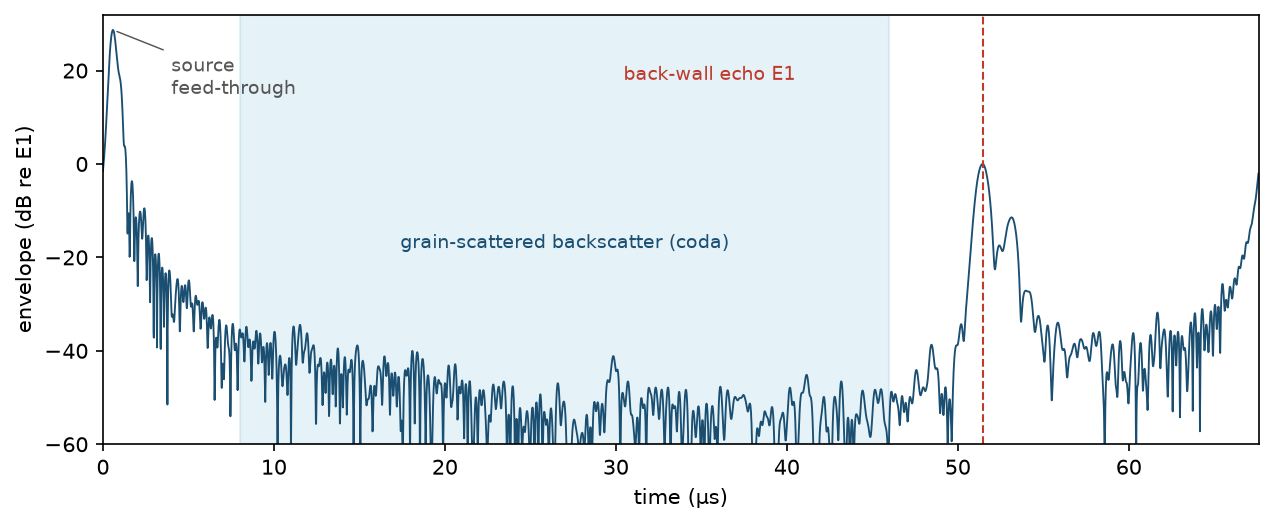
\includegraphics[width=0.95\textwidth]{figures/trace-anatomy.png}
  \caption{A clean 2 MHz reference trace (aligned fabric, envelope in
    dB relative to E1): source feed-through, the grain-scattered
    backscatter that fills the record, and the back-wall echo E1 near
    52 microseconds whose time of flight carries the velocity
    observable.}
  \label{fig:trace}
\end{figure} The arc backprojection
view (\cmd{sim/pipeline/}) maps coherent energy in the received
traces back into the disk and is the quickest qualitative check that
a sweep contains structure rather than noise.

\section{The error model}

The error model corrupts ideal simulated acquisitions with the
distortions the physical machine actually exhibits, so inversion
robustness is tested against the right enemies rather than generic
noise. The configurable terms mirror the instrument's error budget:
timing jitter, per-dock coupling variation (the re-seated couplant
film), angular error on the commanded azimuth, slow drift across a
sweep (the thermal term the machine corrects with reference
revisits), and additive noise at the receiver.

Because the same fabric can be re-acquired with different error
draws, the pipeline separates what limits recovery: fabric ambiguity
(Chapter~\ref{ch:analysis}), acquisition corruption, or both. The
studio's gated workflow enforces the order: an error model is chosen
before acquisition, and the acquired dataset records the model that
produced it.


\chapter{Analysis and inversion}\label{ch:analysis}
\section{Fabric inversion}

The primary observable is the azimuthal velocity pattern
$v(\varphi)$, read through the E1 time of flight
(Figure~\ref{fig:sweepobs}), and the primary inversion
(\cmd{sim/model/fit\_fabric.py}, \cmd{fit\_sweep.py}) recovers fabric
parameters from it in two stages: a coarse global search over fabric
strength and direction followed by local refinement, which avoids the
local minima that a direct descent on the periodic $2\varphi$ pattern
invites. The fit reports the recovered eigenvalue and fast-axis
azimuth with residuals, and the sweep-level tooling fits entire
simulated campaigns unattended.

\begin{figure}[htb]
  \centering
  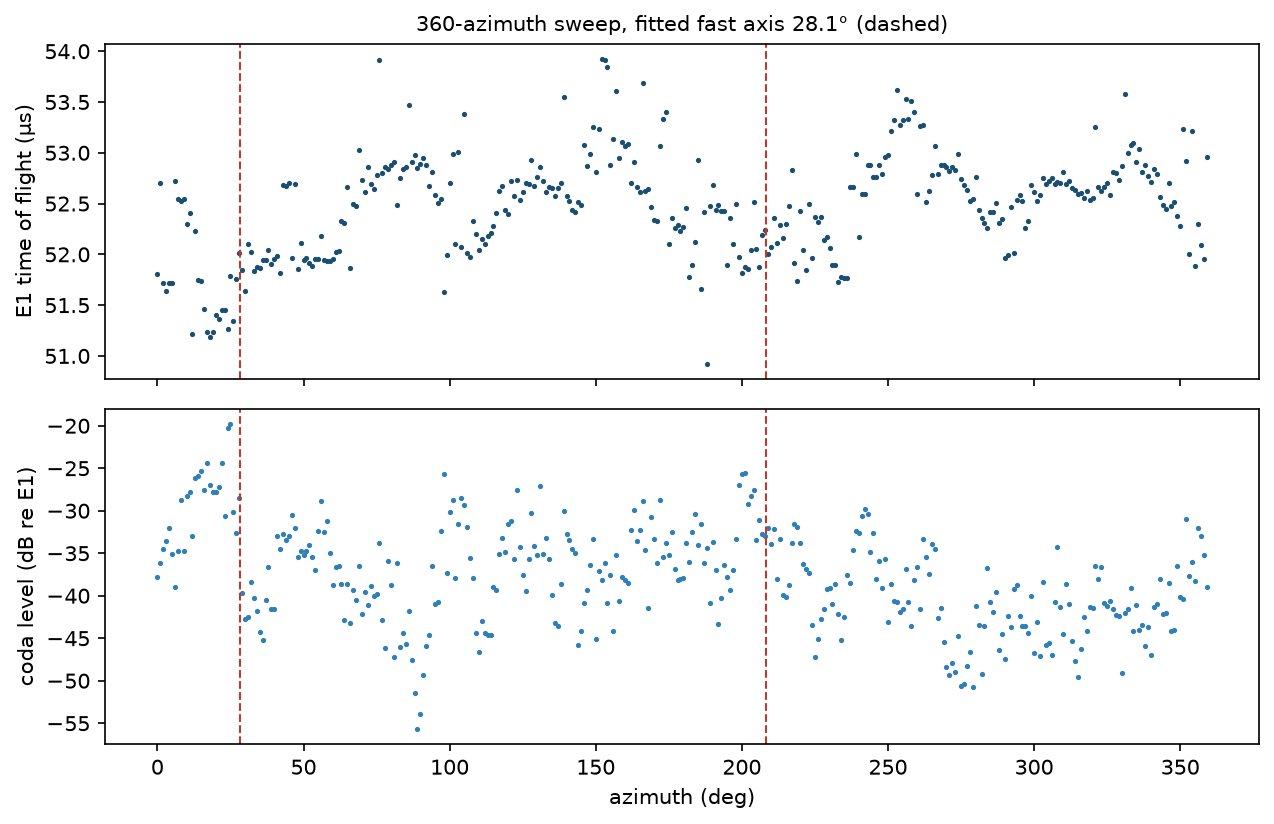
\includegraphics[width=0.95\textwidth]{figures/sweep-observables.png}
  \caption{A complete 360-azimuth full-wave sweep: E1 time of flight
    (top) and coda level (bottom) against azimuth. The
    second-harmonic time-of-flight pattern and the coda elevation
    around the fabric axis are both visible by eye; dashed lines mark
    the fitted fast axis.}
  \label{fig:sweepobs}
\end{figure}

Beyond the single bulk fit, a gridded inversion divides the disk into
regions and inverts per-area fabric, with a daemon that processes
sweeps as they complete. Its purpose is honesty about spatial
resolution: a diametral measurement integrates along chords, so
per-area recovery is only meaningfully constrained where chords
cross, and the gridded results quantify that rather than assert it.

\section{The scattered field}

A large fraction of the analysis layer interrogates the incoherent
part of the received signal: the grain-scattered coda that arrives
after the specular echoes. The central question was whether the coda
carries usable fabric information of its own.

The settled model is geometric: the late field is described by
contrast-weighted facet reflections, in which each grain-boundary
facet contributes according to its orientation and the acoustic
contrast across it. The model was accepted only after it survived
three independent controls (its supporting modules and their expected
numbers live under \cmd{sim/analysis/}, primarily the facet-model
and physical-optics themes), and it explains the observed coda
statistics without invoking fabric-specific propagation effects.

That last clause is the important one, and it is a negative result:
see the next section.

\section{Negative results are kept}

The repository retains every serious attempt that failed, with the
measurements that killed it, because the paper's claims about what
the measurement can do rest equally on demonstrations of what it
cannot.

The flagship negative result concerns the coda: multiple independent
routes (correlation structure, frequency behaviour, channel
statistics, cross-fabric comparisons) each failed to extract fabric
information from the scattered tail beyond what the coherent
$2\varphi$ velocity pattern already provides. The conclusion, tested
from four directions before being accepted, is that on this
geometry the coda does not measure fabric; what survives is the
facet-scattering description of the previous section. The analysis
modules behind each route remain runnable, docstrings recording what
they were expected to show and what they showed instead.

Practical guidance for anyone extending the work: before pursuing a
new signal path, read \cmd{sim/analysis/README.md} and the negative
results first. The most tempting ideas have usually been tried, and
the stored evidence says exactly how they died.


\chapter{Software}\label{ch:software}
\section{Repository architecture}

The code is organised by role, and \cmd{sim/README.md} is the
authoritative file-by-file map; this section gives the shape.

\begin{description}
  \item[sim/core/] the solver and specimen machinery: the
    label-indexed anisotropic FDTD solver, the pseudospectral
    solver, the specimen builder, rotation machinery, and the
    bit-equivalence gate.
  \item[sim/model/] forward models and inversion: the born ladder,
    the fabric and sweep fits, the gridded inversion and its daemon,
    and the ray model the studio uses.
  \item[sim/pipeline/] drivers: the resumable sweep engine, trace
    lab, arc backprojection and visualisation.
  \item[sim/fe\_crosscheck/] the independent finite-element arbiter
    and its archived cross-check rounds.
  \item[sim/fw\_checks/ and sim/validation/] the validation chain of
    Chapter~\ref{ch:forward}.
  \item[sim/analysis/] roughly 75 analysis modules with their stored
    results, grouped by theme, each self-contained and runnable from
    its own directory.
  \item[sim/ref/, sim/runs/, sim/results/, sim/figures/] reference
    traces, batch campaign drivers, stored campaign results, and the
    paper's figure scripts.
  \item[gui/] the Streamlit studio, the sweep tab, and the launcher
    runtime scripts.
  \item[vendor/] vendored dependencies, so the repository is
    self-contained.
\end{description}

Two conventions hold everywhere: modules read stored inputs relative
to their own location, so they run from their own directory with no
environment setup; and expected outputs are recorded in docstrings,
so checking a module means running it and comparing.

\section{The studio GUI}

The GUI (\cmd{gui/app.py}, Streamlit) presents the pipeline as a
gated workflow across tabs: Specimen \& Fabric, Probe \& Excitation,
Error model, Acquisition, then Backscatter and COF reconstruction,
the last two unlocking only once acquired data exists in the
session. The FW sweep tab (\cmd{gui/sweep\_tab.py}) configures,
launches and monitors full-wave sweeps through the sweep engine.

The specimen views are worth knowing about even for command-line
users, since they are the fastest way to sanity-check a fabric: a 3D
per-grain isosurface rendering coloured by c-axis, a c-axis vector
field, an equal-area pole figure with orientation-tensor
eigenvalues, and 2D slices of the grain and azimuth fields.

One engineering note recorded here because it is invisible in the
code's behaviour and expensive to rediscover: the GUI never probes
the GPU at import time. Streamlit executes the script in a worker
thread, and initialising CUDA off the main thread crashes the whole
server without a traceback; the backend is therefore detected by
inspection (is cupy importable, is a CUDA path configured) and the
solvers touch the driver only when actually run.

\section{Data layout and environments}

\subsection{Where data lives}

\begin{description}
  \item[out/sweeps/] one directory per sweep session: a
    \cmd{config.json}, one trace archive per completed azimuth, and
    fit results. Resumable and analysable while incomplete.
  \item[out/tesscache/, out/observables/] the tessellation cache and
    observable matrices, regenerated on demand.
  \item[sim/analysis/*/ (stored npz)] each analysis theme stores its
    own results beside its code.
  \item[sim/ref/] the clean reference traces behind the paper's
    figures.
\end{description}

None of \cmd{out/} is version-controlled; it is deposited with the
paper. \cmd{DATA\_MANIFEST.md} records the mapping. The large
finite-element meshes are not versioned; the meshing scripts rebuild
them if rerun.

\subsection{Environments}

Three usage tiers, in increasing weight:

\begin{enumerate}
  \item \textbf{Analysis only} (no GPU): the pinned numpy and scipy
    of \cmd{requirements.txt}. Every stored result reproduces on
    CPU.
  \item \textbf{GUI}: the pinned set plus streamlit and plotly
    (matplotlib is already required for figures). The launcher's
    private runtime installs exactly this.
  \item \textbf{New solver runs}: additionally CUDA and cupy. Only
    needed to regenerate sweeps or reference traces.
\end{enumerate}

\subsection{The manual}

This document builds from \cmd{docs/} with \cmd{build.ps1} (XeLaTeX,
two passes). Each chapter is a numbered folder and each section a
separate file, so updates touch a single small file.


\chapter*{Related publications}
\addcontentsline{toc}{chapter}{Related publications}

\begin{itemize}
  \item J. Graves, S. Harput, B. Lishman.
    \emph{A Finite-Difference Simulation Framework for Ultrasonic
    Crystal Orientation Fabric Estimation in Ice: Timing Methodology,
    Forward Model Selection, and the Cram\'er-Rao Accuracy Limit.}
    IEEE International Ultrasonics Symposium, 2026 (accepted). The
    paper this repository underpins.
  \item J. Graves, S. Harput, B. Lishman.
    \emph{Non-Destructive Ultrasonic Estimation of Ice Crystal
    Orientation Fabric: Multi-Frequency Experimental Validation and
    Failure Mode Characterisation.} IEEE International Ultrasonics
    Symposium, 2026 (accepted). The experimental companion, measured
    on the physical scanner.
  \item J. Graves, B. Lishman, S. Harput.
    \emph{Measuring Predominant Orientations of Ice Crystal Fabrics
    From Ultrasonic Measurements of Ice Cores.} Preprint.
  \item J. Graves, B. Lishman, S. Harput.
    \emph{Determining the Grain Geometry From Ultrasonic Measurements
    of Large-Grained Temperate Ice Cores.} IEEE International
    Ultrasonics Symposium, 2023.
    \href{https://doi.org/10.1109/ius51837.2023.10307539}{doi:10.1109/ius51837.2023.10307539}.
\end{itemize}

The full list is maintained at
\href{https://jeromegraves.com/\#publications}{jeromegraves.com}.


\end{document}
